\section{Task level modeling}

\begin{table}[H]
\centering
\begin{tabularx}{\textwidth}{|l|X|r|r|}
\hline
\textbf{Position} & \textbf{Description} & \textbf{Salary} & \textbf{Normalized Salary} \\
\hline
Clerk & & \$52,000.00 & 1.00 \\
\hline
Data analyst & & \$60,000.00 & 1.15 \\
\hline
ML engineer & & \$130,000.00 & 2.50 \\
\hline
Data scientist & & \$123,000.00 & 2.37 \\
\hline
Domain expert (Neurologist) & & \$267,000.00 & 5.13 \\
\hline
\multicolumn{2}{|l|}{\textbf{Minimum}} & \$52,000.00 & 1.00 \\
\hline
\end{tabularx}
\caption{Salary and normalized salary for each position}
\label{table:salary}
\end{table}

\subsection{Segregation system}

\subsubsection{Check data balancing}

The task is performed by a Data Analyst.

\begin{figure}[H]
\centering
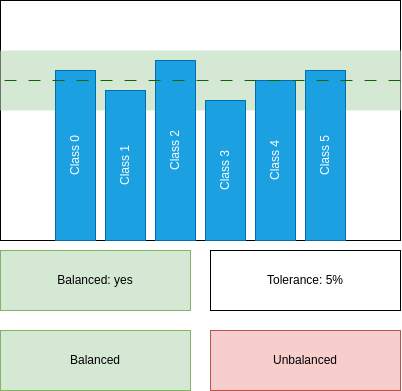
\includegraphics[width=0.8\textwidth]{figures/check_data_balancing.png}
\caption{"Check data balancing" mock-up form}
\end{figure}

\begin{table}[H]
\centering
\begin{tabularx}{\textwidth}{|X|c|c|c|c|}
\hline
\textbf{Step} & \textbf{O} & \textbf{CL} & \textbf{S} & \textbf{SC} \\
\hline
\textbf{1} \textbf{ACTOR} opens "Check data balancing" form. & 1 & 1 & 1.15 & 1.15 \\
\hline
\textbf{2} \textbf{SYSTEM} shows the report. & & & & \\
\hline
\textbf{3} \textbf{SYSTEM} shows a hint whether the data is balanced or not. & & & & \\
\hline
\textbf{4} \textbf{ACTOR} checks threshold in the UI. & 1 & 2 & 1.15 & 2.30 \\
\hline
\textbf{5} \textbf{FOR EACH} column in the report: & 5 & & & \\
\hline
\textbf{5.1} \textbf{IF} the column is not within the displayed threshold. & 4 & & & \\
\hline
\textbf{5.1.1} \textbf{THEN} the data is not balanced. & 4 & & & \\
\hline
\textbf{6.1} \textbf{IF} the data is balanced. & 0.2 & & & \\
\hline
\textbf{6.1.1} \textbf{ACTOR} clicks "Balanced" button. & 0.2 & 1 & 1.15 & 0.23 \\
\hline
\textbf{6.2} \textbf{ELSE} & 0.8 & & & \\
\hline
\textbf{6.2.1} \textbf{ACTOR} clicks "Unbalanced" button. & 0.8 & 1 & 1.15 & 0.92 \\
\hline
\textbf{7} \textbf{SYSTEM} shows a confirmation dialog. & & & & \\
\hline
\textbf{8} \textbf{ACTOR} closes the form. & 1 & 1 & 1.15 & 1.15 \\
\hline
\multicolumn{4}{|r|}{Human task cost} & 5.75 \\
\hline
\end{tabularx}
\caption{Detailed use case for "Check data balancing" task\\ 
 O - Occurrence, CL - Cognitive Level, S - Normalized Salary, SC - Step Cost}
\label{table:check_data_balancing}
\end{table}

\subsubsection{Check input coverage}

The task is performed by a Data Analyst.

\begin{figure}[H]
\centering
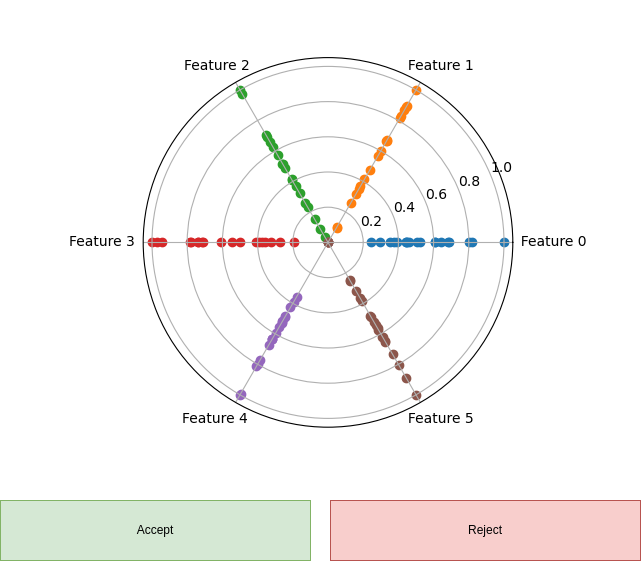
\includegraphics[width=0.8\textwidth]{figures/check_input_coverage.png}
\caption{"Check input coverage" mock-up form}
\end{figure}

\begin{table}[H]
\centering
\begin{tabularx}{\textwidth}{|X|c|c|c|c|}
\hline
\textbf{Step} & \textbf{O} & \textbf{CL} & \textbf{S} & \textbf{SC} \\
\hline
\textbf{1} \textbf{ACTOR} opens "Check input coverage" form. & 1 & 1 & 1.15 & 1.15 \\
\hline
\textbf{2} \textbf{SYSTEM} shows a radar scatter plot of the input distribution. & & & & \\
\hline
\textbf{3} \textbf{FOR EACH} radius in the radar scatter plot: & 5 & & & \\
\hline
\textbf{3.1} \textbf{IF} the distribution is not uniform as expected. & 3.33 & 4 & 1.15 & 15.32\\
\hline
\textbf{3.1.1} \textbf{THEN} the input coverage is not satisfied. & 3.33 & & & \\
\hline
\textbf{4.1} \textbf{IF} the input coverage is satisfied. & 0.33 & & & \\
\hline
\textbf{4.1.1} \textbf{ACTOR} clicks "Accept" button. & 0.33 & 1 & 1.15 & 0.38\\
\hline
\textbf{4.2} \textbf{ELSE} & 0.66 & & & \\
\hline
\textbf{4.2.1} \textbf{ACTOR} clicks "Reject" button. & 0.66 & 1 & 1.15 & 0.77\\
\hline
\textbf{5} \textbf{SYSTEM} shows a confirmation dialog. & & & & \\
\hline
\textbf{6} \textbf{ACTOR} closes the form. & 1 & 1 & 1.15 & 1.15 \\
\hline
\multicolumn{4}{|r|}{Human task cost} & 18.77\\
\hline
\end{tabularx}
\caption{Detailed use case for "Check input coverage" task\\ 
O - Occurrence, CL - Cognitive Level, S - Normalized Salary, SC - Step Cost}
\label{table:check_input_coverage}
\end{table}

\subsubsection{Configure Segregation System}
This task is performed by a ML Engineer.

\begin{figure}[H]
\centering
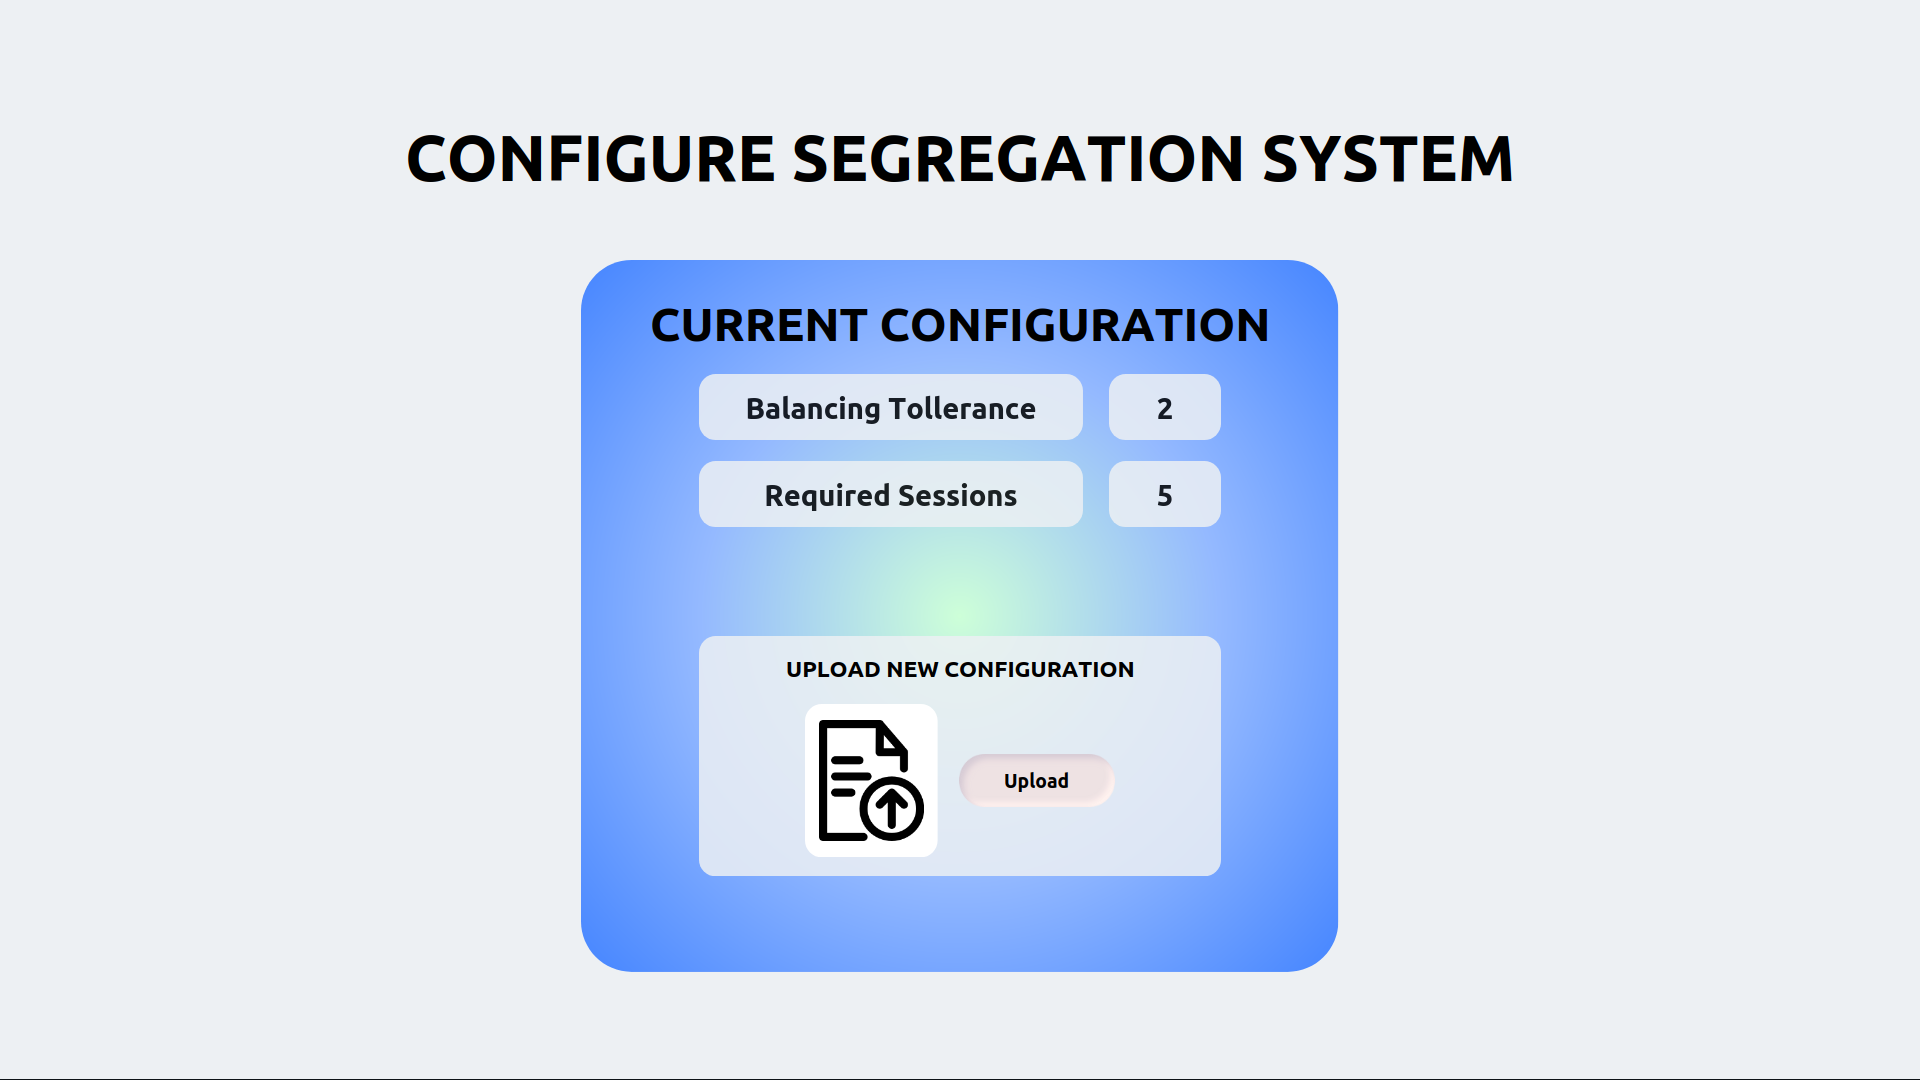
\includegraphics[width=0.8\textwidth]{docs/figures/ui_configure_segregation.png}
\caption{"Configure Segregation System" mock-up form}
\end{figure}

\begin{table}[H]
\centering
\begin{tabularx}{\textwidth}{|X|c|c|c|c|}
\hline
\textbf{Step} & \textbf{O} & \textbf{CL} & \textbf{S} & \textbf{SC} \\
\hline
\textbf{1} \textbf{ACTOR} opens the "Configure Segregation System" form. &  & & & \\
\hline
\textbf{2} \textbf{SYSTEM} displays the current configuration and the "Upload" button.& & & & \\
\hline
\textbf{3} \textbf{ACTOR} push the "Upload" button and upload the configuration file. & & & &\\
\hline
\textbf{4} \textbf{SYSTEM} shows a confirmation message. & & & & \\
\hline
\textbf{5} \textbf{ACTOR} closes the form. & & & & \\
\hline
\multicolumn{4}{|r|}{Human task cost} & \\
\hline
\end{tabularx}
\caption{Detailed use case for "Configure Segregation" task\\ 
O - Occurrence, CL - Cognitive Level, S - Normalized Salary, SC - Step Cost}
\label{table:configure_client_side}
\end{table}
\subsection{Development system}

\subsubsection{Set iteration number}

The task is performed by a ML engineer.

\begin{figure}[H]
\centering
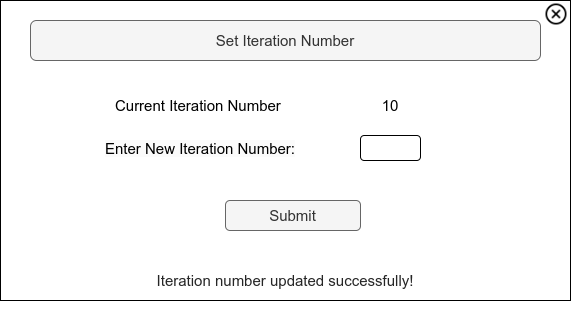
\includegraphics[width=0.8\textwidth]{figures/set_iteration_number.png}
\caption{"Set iteration number" mock-up form}
\end{figure}

\begin{table}[H]
\centering
\begin{tabularx}{\textwidth}{|X|c|c|c|c|}
\hline
\textbf{Step} & \textbf{O} & \textbf{CL} & \textbf{S} & \textbf{SC} \\
\hline
\textbf{1} \textbf{ACTOR} opens "Set Iteration Number" form. & 1 & 1 & 2.5 & 2.5 \\
\hline
\textbf{2} \textbf{SYSTEM} displays the current iteration number. & & & & \\
\hline
\textbf{3} \textbf{ACTOR} inputs the desired number of iterations. & 1 & 3 & 2.5 & 7.5 \\
\hline
\textbf{4} \textbf{ACTOR} clicks "Submit" button to confirm the iteration number. & 1 & 1 & 2.5 & 2.5 \\
\hline
\textbf{5} \textbf{SYSTEM} shows a confirmation dialog. & & & & \\
\hline
\textbf{6} \textbf{ACTOR} closes the form. & 1 & 1 & 2.5 & 2.5 \\
\hline
\multicolumn{4}{|r|}{Human task cost} &  15 \\
\hline
\end{tabularx}
\caption{Detailed use case for "Set iteration number" task\\ 
O - Occurrence, CL - Cognitive Level, S - Normalized Salary, SC - Step Cost}
\label{table:set_iteration_number}
\end{table}

\subsubsection{Check learning report}

The task is performed by a ML engineer.

\begin{figure}[H]
\centering
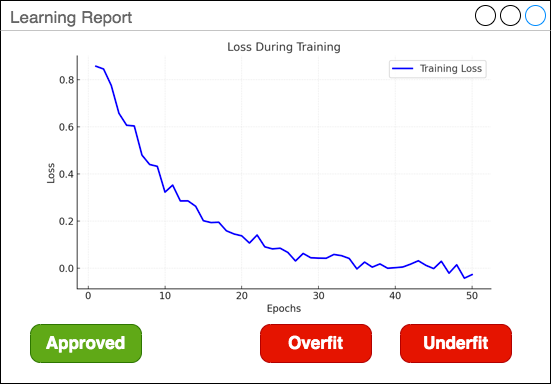
\includegraphics[width=0.8\textwidth]{figures/check_learning_report.png}
\caption{"Check learning report" mock-up form}
\end{figure}

\begin{table}[H]
\centering
\begin{tabularx}{\textwidth}{|X|c|c|c|c|}
\hline
\textbf{Step} & \textbf{O} & \textbf{CL} & \textbf{S} & \textbf{SC} \\
\hline
\textbf{1} \textbf{ACTOR} opens "Check training report" form. & 1 & 1 & 2.50 & 2.50 \\
\hline
\textbf{2} \textbf{SYSTEM} shows the training loss curve. & & & & \\
\hline
\textbf{3.1} \textbf{IF} the loss is flat for at least half of the iterations: & 0.4 & 3 & 2.50 & 3.00 \\
\hline
\textbf{3.1.1} \textbf{THEN} \textbf{ACTOR} clicks "Overfit" button. & 0.4 & 1 & 2.50 & 1.00 \\
\hline
\textbf{3.2} \textbf{IF} the loss is not flat at the end of the iterations: & 0.4 & 3 & 2.50 & 3.00 \\
\hline
\textbf{3.2.1} \textbf{THEN} \textbf{ACTOR} clicks "Underfit" button. & 0.4 & 1 & 2.50 & 1.00 \\
\hline
\textbf{3.3} \textbf{ELSE} & 0.2 & 3 & 2.50 & 1.50 \\
\hline
\textbf{3.3.1} \textbf{ACTOR} clicks "Approved" button. & 0.2 & 1 & 2.50 & 0.50 \\
\hline
\textbf{4} \textbf{SYSTEM} shows a confirmation dialog. & & & & \\
\hline
\textbf{5} \textbf{ACTOR} closes the form. & 1 & 1 & 2.50 & 2.50 \\
\hline
\multicolumn{4}{|r|}{Human task cost} & 15.00 \\
\hline
\end{tabularx}
\caption{Detailed use case for "Check training report" task\\ 
O - Occurrence, CL - Cognitive Level, S - Normalized Salary, SC - Step Cost}
\label{table:check_training_report}
\end{table}

\subsubsection{Check validation report}

This task is performed by a ML engineer.

\begin{figure}[H]
\centering
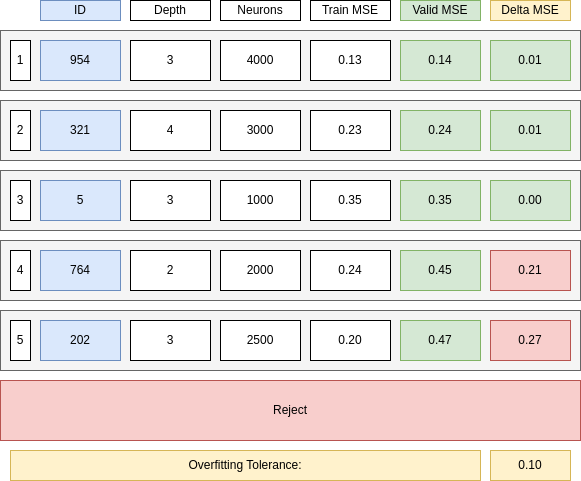
\includegraphics[width=0.8\textwidth]{figures/check_validation_report.png}
\caption{"Check validation report" mock-up form}
\end{figure}

\begin{table}[H]
\centering
\begin{tabularx}{\textwidth}{|X|c|c|c|c|}
\hline
\textbf{Step} & \textbf{O} & \textbf{CL} & \textbf{S} & \textbf{SC} \\
\hline
\textbf{1} \textbf{ACTOR} opens "Check validation report" form. & 1 & 1 & 2.5 & 2.5 \\
\hline
\textbf{2} \textbf{SYSTEM} shows the best 5 models sorted by increasing Validation Loss. & & & & \\
\hline
\textbf{3} \textbf{FOR EACH} model in the list: & 5 & & & \\
\hline
\textbf{3.1} \textbf{IF} the model Validation Loss minus the Training Loss is less than the Overfitting Tolerance and the Best Model is not selected. & 1 & 2 & 2.5 & 5 \\
\hline
\textbf{3.1.1} \textbf{THEN} select the model as the Best Model. & 1 & 1 & 2.5 & 2.5 \\
\hline
\textbf{4} \textbf{FOR EACH} model in the list: & 4 & & & \\
\hline
\textbf{4.1} \textbf{IF} the model is not the Best Model and the Validation Loss minus the Training Loss is less than the Overfitting Tolerance and the Second Best Model is not selected. & 1 & 2 & 2.5 & 5 \\
\hline
\textbf{4.1.1} \textbf{THEN} select the model as the Second Best Model. & 1 & 1 & 2.5 & 2.5 \\
\hline
\textbf{5.1} \textbf{IF} the Best Model is not selected. & 0.05 & 1 & 2.5 & 0.125 \\
\hline
\textbf{5.1.1} \textbf{ACTOR} clicks "Reject" button. & 0.05 & 1 & 2.5 & 0.125\\
\hline
\textbf{5.2} \textbf{ELSE IF} the Second Best Model is not selected or the Validation Loss of the Second Best Model is one order of magnitude greater than the Validation Loss of the Best Model. & 0.3 & 3 & 2.5 & 2.25 \\
\hline
\textbf{5.2.1} \textbf{ACTOR} clicks on the Best Model. & 0.3 & 1 & 2.5 & 0.75 \\
\hline
\textbf{5.3} \textbf{ELSE} & 0.65 & 3 & 2.5 & 4.875 \\
\hline
\textbf{5.3.1} \textbf{ACTOR} clicks on the least complex model among the Best Model and the Second Best Model. & 0.65 & 3 & 2.5 & 4.875 \\
\hline
\textbf{6} \textbf{SYSTEM} shows a confirmation dialog. & & & & \\
\hline
\textbf{7} \textbf{ACTOR} closes the form. & 1 & 1 & 2.5 & 2.5 \\
\hline
\multicolumn{4}{|r|}{Human task cost} & 32.91 \\
\hline
\end{tabularx}
\caption{Detailed use case for "Check validation report" task\\ 
O - Occurrence, CL - Cognitive Level, S - Normalized Salary, SC - Step Cost}
\label{table:check_validation_report}
\end{table}

\subsubsection{Check test results}

This task is performed by a ML engineer.

\begin{figure}[H]
\centering
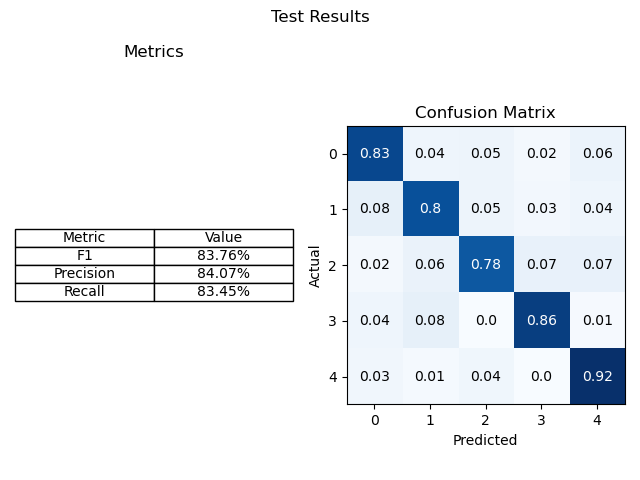
\includegraphics[width=0.8\textwidth]{figures/check_test_results.png}
\caption{"Check test results" mock-up form}
\end{figure}

\begin{table}[H]
\centering
\begin{tabularx}{\textwidth}{|X|c|c|c|c|}
\hline
\textbf{Step} & \textbf{O} & \textbf{CL} & \textbf{S} & \textbf{SC} \\
\hline
\textbf{1} \textbf{ACTOR} opens "Check test results" form. & 1 & 1 & 2.5 & 2.5 \\
\hline
\textbf{2} \textbf{SYSTEM} shows the test results. & & & & \\
\hline
\textbf{3} \textbf{ACTOR} checks if the difference between the test results and the validation results is within overfitting tolerance. & 1 & 2 & 2.5 & 5 \\
\hline
\textbf{4.1} \textbf{IF} the test results is not satisfactory. & 0.01 & & & \\
\hline
\textbf{4.1.1} \textbf{ACTOR} clicks "Reject" button. & 0.01 & 1 & 2.5 & 0.025 \\
\hline
\textbf{4.2} \textbf{ELSE} & 0.99 & & & \\
\hline
\textbf{4.2.1} \textbf{ACTOR} clicks "Approve" button. & 0.99 & 1 & 2.5 & 2.475 \\
\hline
\textbf{5} \textbf{SYSTEM} shows a confirmation dialog. & & & & \\
\hline
\textbf{6} \textbf{ACTOR} closes the form. & 1 & 1 & 2.5 & 2.5 \\
\hline
\multicolumn{4}{|r|}{Human task cost} & 12.5 \\
\hline
\end{tabularx}
\caption{Detailed use case for "Check test results" task\\ 
O - Occurrence, CL - Cognitive Level, S - Normalized Salary, SC - Step Cost}
\label{table:check_test_results}
\end{table}


\subsubsection{Configure Development System}
This task is performed by a ML Engineer.

\begin{figure}[H]
\centering
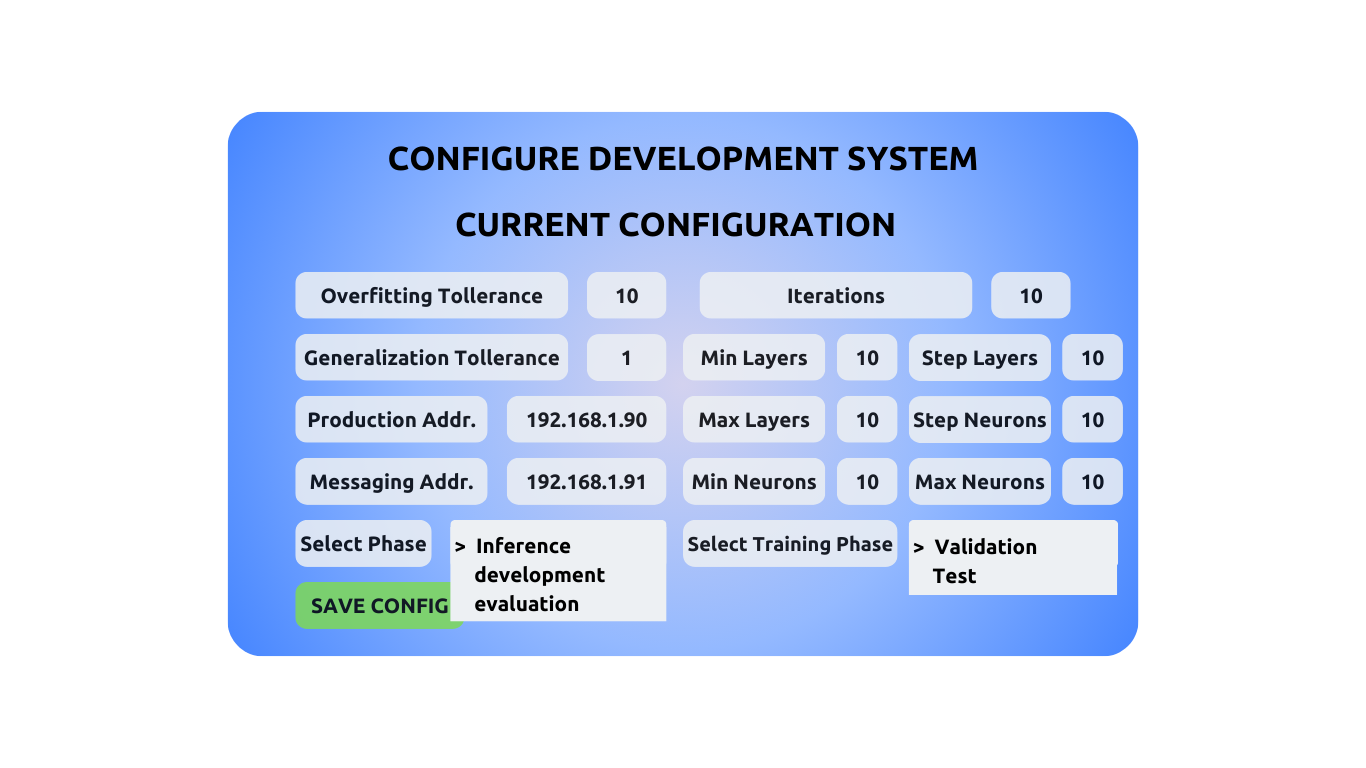
\includegraphics[width=0.8\textwidth]{docs/figures/ui_configure_development.png}
\caption{"Configure Development System" mock-up form}
\end{figure}

\begin{table}[H]
\centering
\begin{tabularx}{\textwidth}{|X|c|c|c|c|}
\hline
\textbf{Step} & \textbf{O} & \textbf{CL} & \textbf{S} & \textbf{SC} \\
\hline
\textbf{1} \textbf{ACTOR} opens the "Configure Development System" form. &  & & & \\
\hline
\textbf{2} \textbf{SYSTEM} displays the current configuration and the "Upload" button.& & & & \\
\hline
\textbf{3} \textbf{ACTOR} push the "Upload" button and upload the configuration file. & & & &\\
\hline
\textbf{4} \textbf{SYSTEM} shows a confirmation message. & & & & \\
\hline
\textbf{5} \textbf{ACTOR} closes the form. & & & & \\
\hline
\multicolumn{4}{|r|}{Human task cost} & \\
\hline
\end{tabularx}
\caption{Detailed use case for "Configure Development" task\\ 
O - Occurrence, CL - Cognitive Level, S - Normalized Salary, SC - Step Cost}
\label{table:configure_client_side}
\end{table}
\subsection{Evaluation system}

\subsubsection{Evaluate classifier performance}
This task is performed by a Data Analyst.

\begin{figure}[H]
\centering
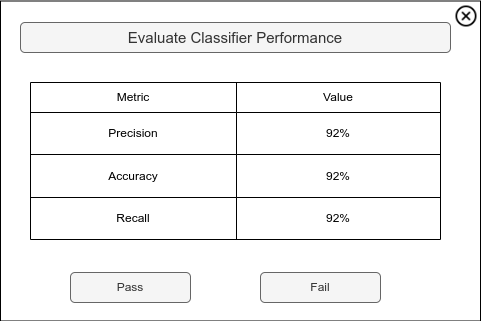
\includegraphics[width=0.8\textwidth]{figures/evaluate_classifier_performance.png}
\caption{"Evaluate Classifier Performance" mock-up form}
\end{figure}

\begin{table}[H]
\centering
\begin{tabularx}{\textwidth}{|X|c|c|c|c|}
\hline
\textbf{Step} & \textbf{O} & \textbf{CL} & \textbf{S} & \textbf{SC} \\
\hline
\textbf{1} \textbf{ACTOR} opens the "Evaluate Classifier Performance" form. & 1 & 1 & 1.15 & 1.15 \\
\hline
\textbf{2} \textbf{SYSTEM} displays a table of sessions with Expert Label (ground truth) and Classifier Label (predicted label). 
The difference between the labels (if any) represents an error. & & & & \\
\hline
\textbf{3} \textbf{ACTOR} reviews the table. & 1 & 4 & 1.15 & 4.60\\
\hline
\textbf{3.1} \textbf{IF} the total errors or consecutive errors exceed their respective thresholds: & 1 & 2 & 1.15 & 2.30 \\
\hline
\textbf{3.1.1} \textbf{ACTOR} clicks the "Fail" button. &0.5 & 1& 1.5&2.30 \\
\hline
\textbf{3.2} \textbf{ELSE} & & & & \\
\hline
\textbf{3.2.1} \textbf{ACTOR} clicks the "Pass" button. &0.5 &1 & 1.5&0.575 \\
\hline
\textbf{4} \textbf{SYSTEM} shows a confirmation dialog. & & & & \\
\hline
\textbf{5} \textbf{ACTOR} closes the form. &1 &1 &1.15 & 1.15\\
\hline
\multicolumn{4}{|r|}{Human task cost} &9.35 \\
\hline
\end{tabularx}
\caption{Detailed use case for "Evaluate Classifier Performance" task\\ 
O - Occurrence, CL - Cognitive Level, S - Normalized Salary, SC - Step Cost}
\label{table:evaluate_classifier_performance}
\end{table}

\subsubsection{Configure Evaluation System}
This task is performed by a ML Engineer.

\begin{figure}[H]
\centering
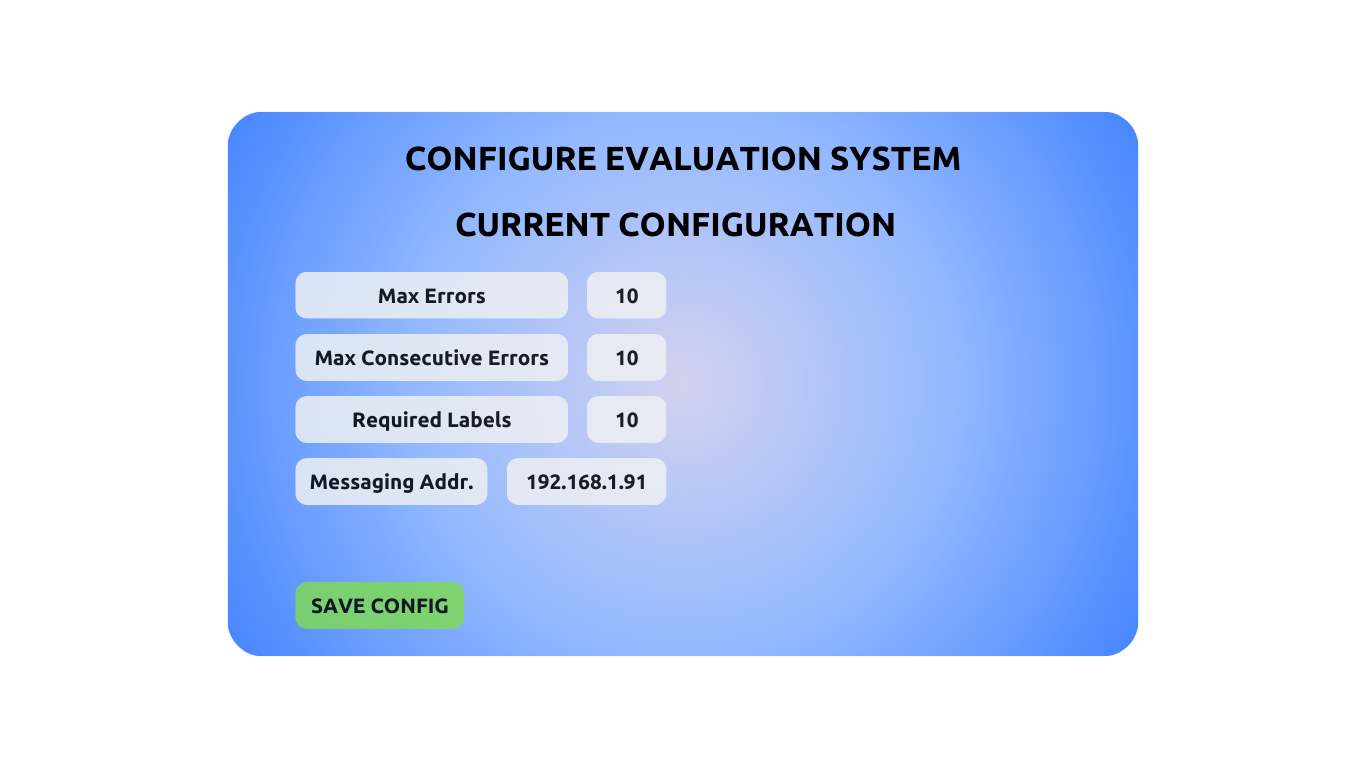
\includegraphics[width=0.8\textwidth]{docs/figures/ui_configure_evaluation.png}
\caption{"Configure Evaluation System" mock-up form}
\end{figure}

\begin{table}[H]
\centering
\begin{tabularx}{\textwidth}{|X|c|c|c|c|}
\hline
\textbf{Step} & \textbf{O} & \textbf{CL} & \textbf{S} & \textbf{SC} \\
\hline
\textbf{1} \textbf{ACTOR} opens the "Configure Evaluation System" form. &  & & & \\
\hline
\textbf{2} \textbf{SYSTEM} displays the current configuration and the "Upload" button.& & & & \\
\hline
\textbf{3} \textbf{ACTOR} push the "Upload" button and upload the configuration file. & & & &\\
\hline
\textbf{4} \textbf{SYSTEM} shows a confirmation message. & & & & \\
\hline
\textbf{5} \textbf{ACTOR} closes the form. & & & & \\
\hline
\multicolumn{4}{|r|}{Human task cost} & \\
\hline
\end{tabularx}
\caption{Detailed use case for "Configure Evaluation" task\\ 
O - Occurrence, CL - Cognitive Level, S - Normalized Salary, SC - Step Cost}
\label{table:configure_client_side}
\end{table}

\subsection{Client-Side Systems}

\subsubsection{Configure Client-Side Systems}
This task is performed by a ML Engineer.

\begin{figure}[H]
\centering
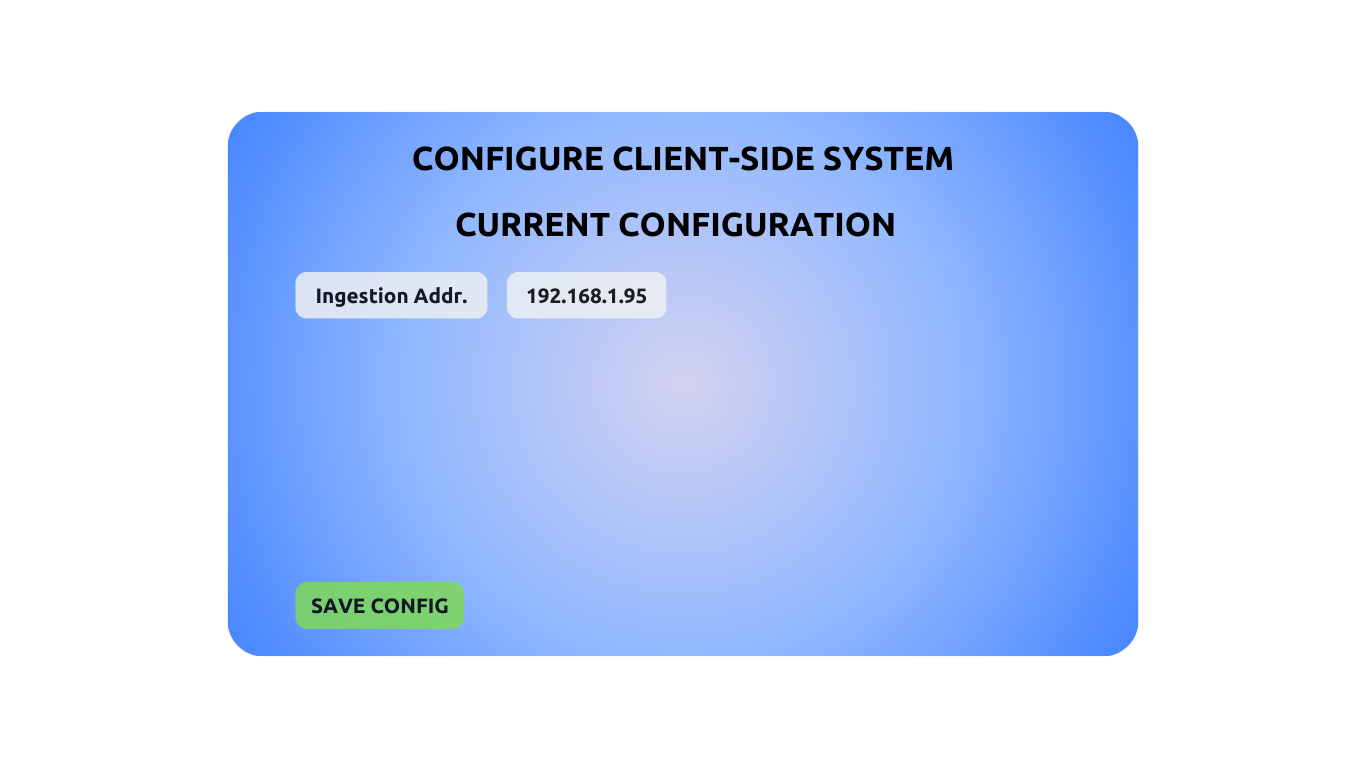
\includegraphics[width=0.8\textwidth]{docs/figures/ui_configure_client-side.png}
\caption{"Configure Client-Side Systems" mock-up form}
\end{figure}

\begin{table}[H]
\centering
\begin{tabularx}{\textwidth}{|X|c|c|c|c|}
\hline
\textbf{Step} & \textbf{O} & \textbf{CL} & \textbf{S} & \textbf{SC} \\
\hline
\textbf{1} \textbf{ACTOR} opens the "Configure Client-Side System" form. &  & & & \\
\hline
\textbf{2} \textbf{SYSTEM} displays the "Upload" button.& & & & \\
\hline
\textbf{3} \textbf{ACTOR} push the "Upload" button and upload the configuration file. & & & &\\
\hline
\textbf{4} \textbf{SYSTEM} shows a confirmation message. & & & & \\
\hline
\textbf{5} \textbf{ACTOR} closes the form. & & & & \\
\hline
\multicolumn{4}{|r|}{Human task cost} & \\
\hline
\end{tabularx}
\caption{Detailed use case for "Configure Client-Side Systems" task\\ 
O - Occurrence, CL - Cognitive Level, S - Normalized Salary, SC - Step Cost}
\label{table:configure_client_side}
\end{table}


\subsection{Production System}

\subsubsection{Configure Production Systems}
This task is performed by a ML Engineer.

\begin{figure}[H]
\centering
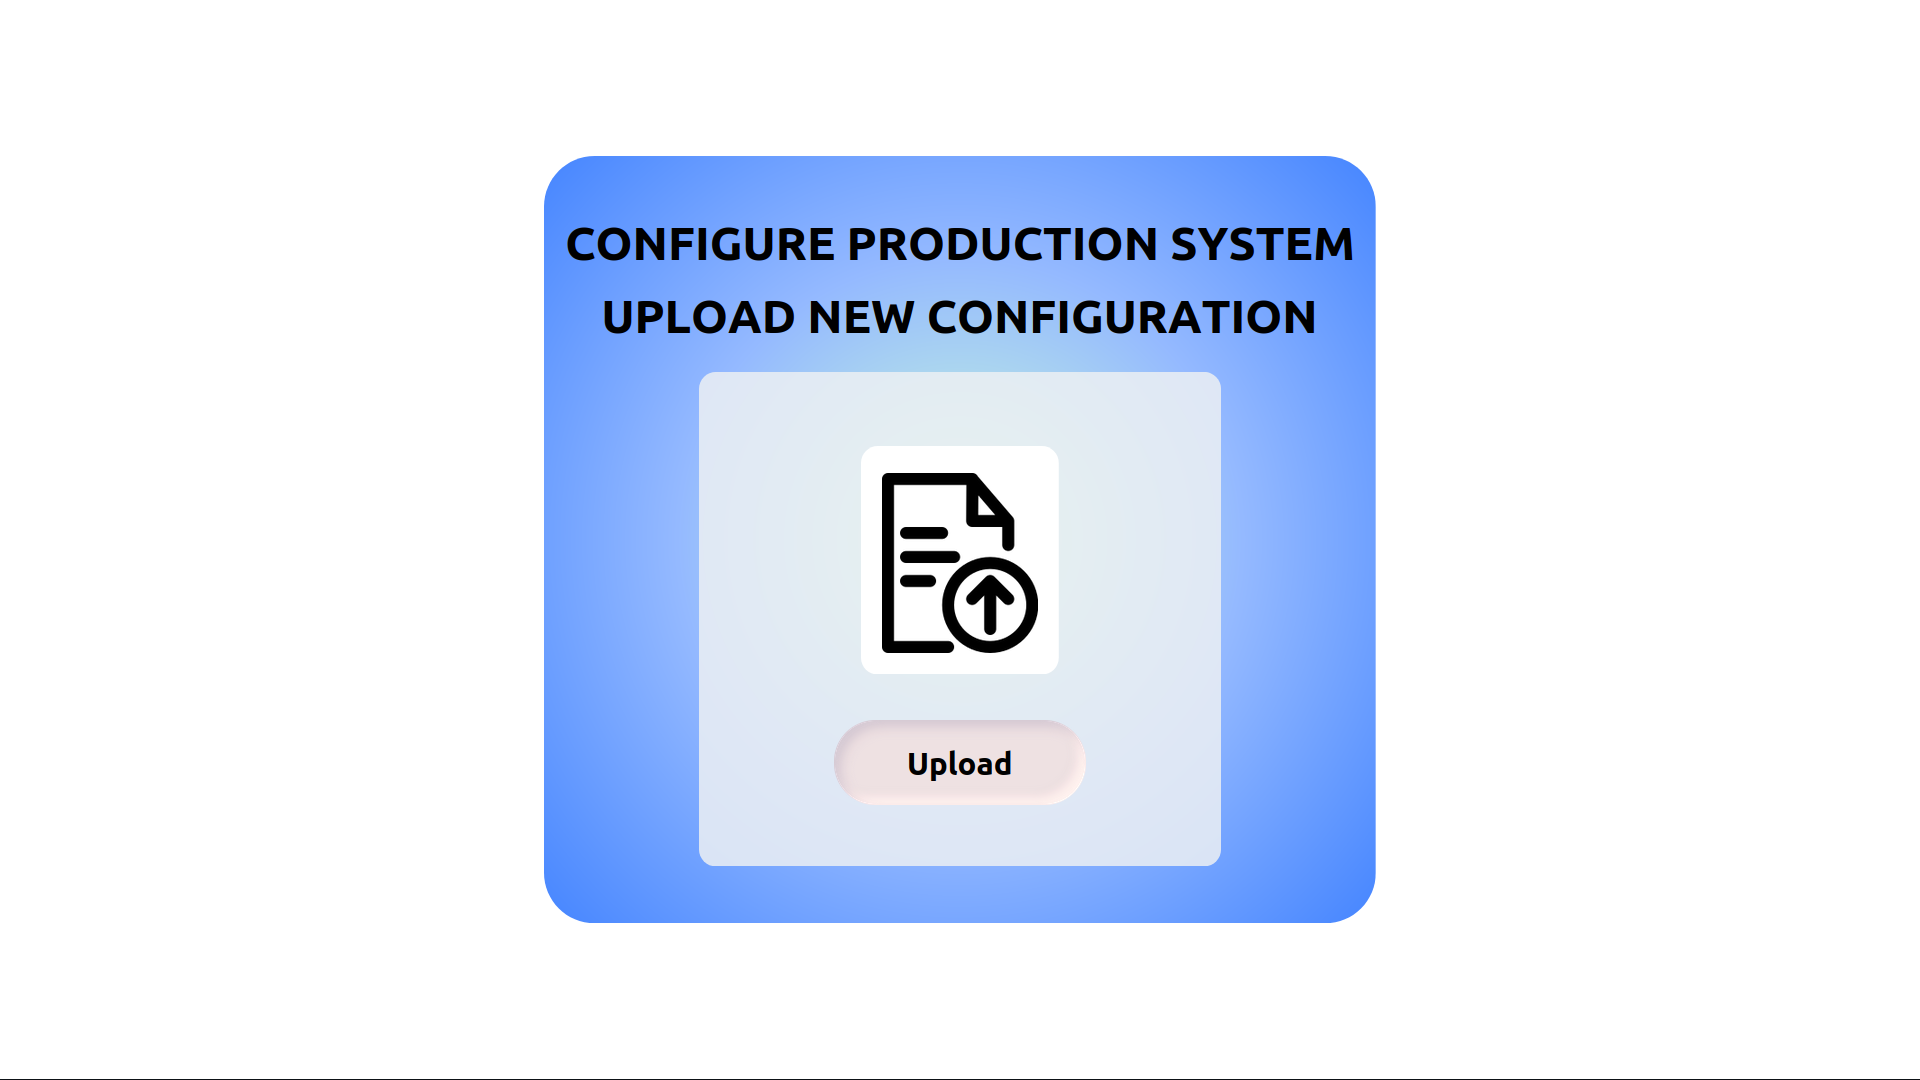
\includegraphics[width=0.8\textwidth]{docs/figures/ui_configure_production.png}
\caption{"Configure Production System" mock-up form}
\end{figure}

\begin{table}[H]
\centering
\begin{tabularx}{\textwidth}{|X|c|c|c|c|}
\hline
\textbf{Step} & \textbf{O} & \textbf{CL} & \textbf{S} & \textbf{SC} \\
\hline
\textbf{1} \textbf{ACTOR} opens the "Configure Production System" form. &  & & & \\
\hline
\textbf{2} \textbf{SYSTEM} displays the "Upload" button.& & & & \\
\hline
\textbf{3} \textbf{ACTOR} push the "Upload" button and upload the configuration file. & & & &\\
\hline
\textbf{4} \textbf{SYSTEM} shows a confirmation message. & & & & \\
\hline
\textbf{5} \textbf{ACTOR} closes the form. & & & & \\
\hline
\multicolumn{4}{|r|}{Human task cost} & \\
\hline
\end{tabularx}
\caption{Detailed use case for "Configure Production" task\\ 
O - Occurrence, CL - Cognitive Level, S - Normalized Salary, SC - Step Cost}
\label{table:configure_client_side}
\end{table}



\subsection{Ingestion System}

\subsubsection{Configure Ingestion System}
This task is performed by a ML Engineer.

\begin{figure}[H]
\centering
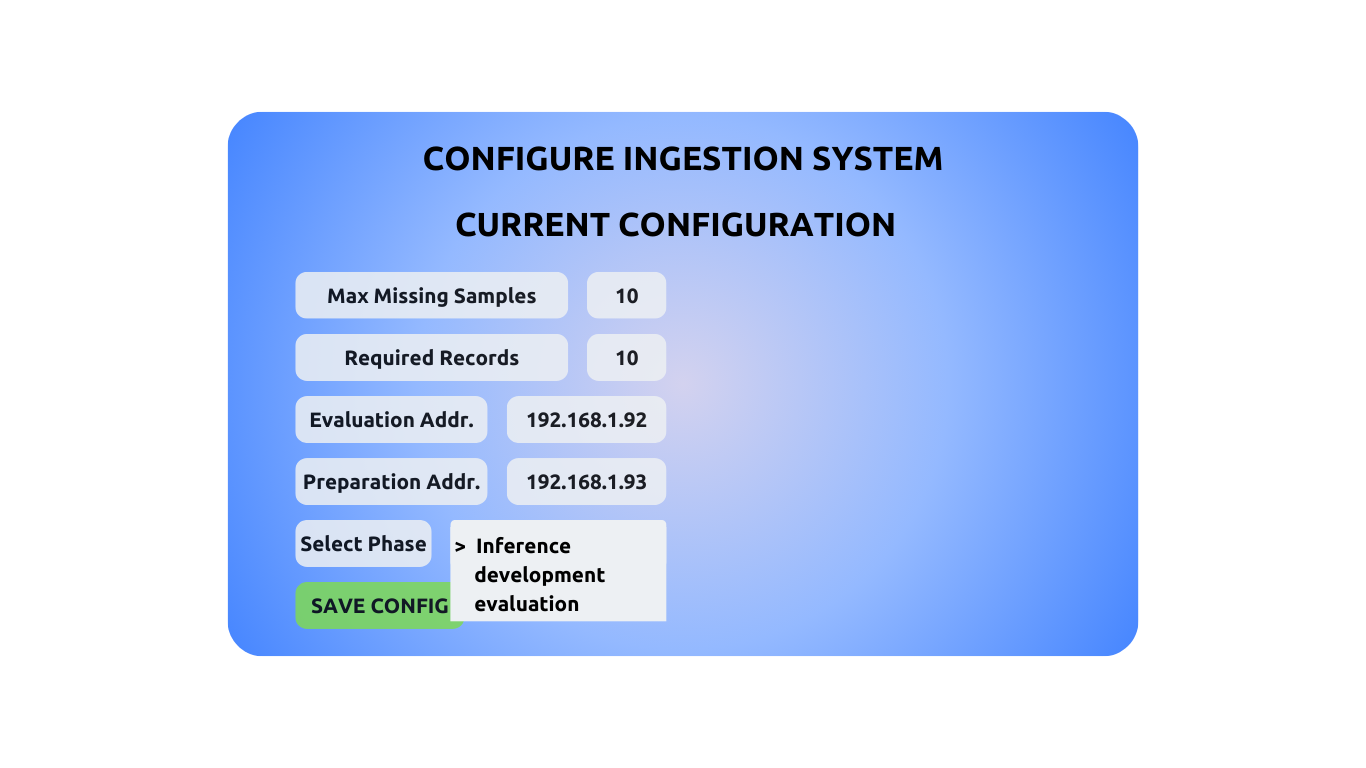
\includegraphics[width=0.8\textwidth]{docs/figures/ui_configure_ingestion.png}
\caption{"Configure Ingestion System" mock-up form}
\end{figure}

\begin{table}[H]
\centering
\begin{tabularx}{\textwidth}{|X|c|c|c|c|}
\hline
\textbf{Step} & \textbf{O} & \textbf{CL} & \textbf{S} & \textbf{SC} \\
\hline
\textbf{1} \textbf{ACTOR} opens the "Configure Ingestion System" form. &  & & & \\
\hline
\textbf{2} \textbf{SYSTEM} displays the current configuration and the "Upload" button.& & & & \\
\hline
\textbf{3} \textbf{ACTOR} push the "Upload" button and upload the configuration file. & & & &\\
\hline
\textbf{4} \textbf{SYSTEM} shows a confirmation message. & & & & \\
\hline
\textbf{5} \textbf{ACTOR} closes the form. & & & & \\
\hline
\multicolumn{4}{|r|}{Human task cost} & \\
\hline
\end{tabularx}
\caption{Detailed use case for "Configure Ingestion" task\\ 
O - Occurrence, CL - Cognitive Level, S - Normalized Salary, SC - Step Cost}
\label{table:configure_client_side}
\end{table}






\subsection{Preparation System}

\subsubsection{Configure Preparation System}
This task is performed by a ML Engineer.

\begin{figure}[H]
\centering
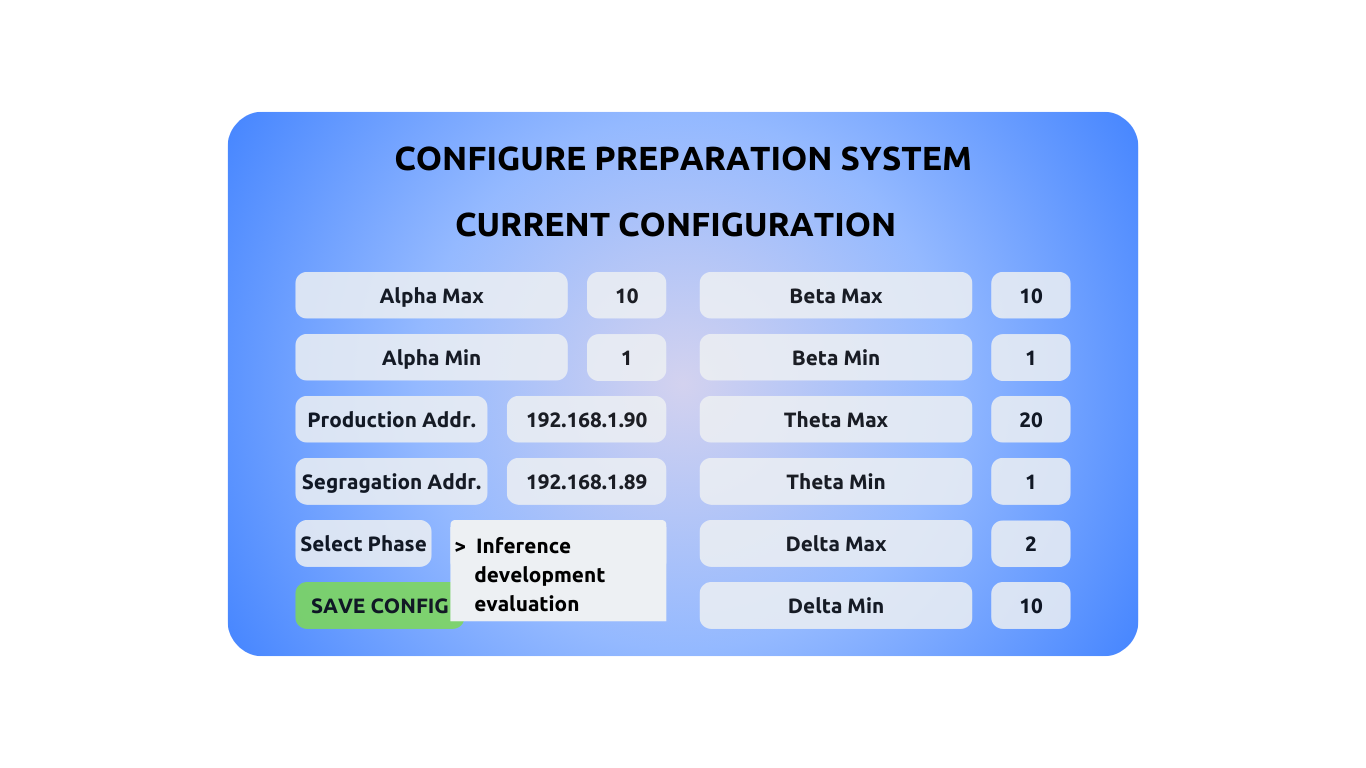
\includegraphics[width=0.8\textwidth]{docs/figures/ui_configure_preparation.png}
\caption{"Configure Preparation System" mock-up form}
\end{figure}

\begin{table}[H]
\centering
\begin{tabularx}{\textwidth}{|X|c|c|c|c|}
\hline
\textbf{Step} & \textbf{O} & \textbf{CL} & \textbf{S} & \textbf{SC} \\
\hline
\textbf{1} \textbf{ACTOR} opens the "Configure Preparation System" form. &  & & & \\
\hline
\textbf{2} \textbf{SYSTEM} displays the current configuration and the "Upload" button.& & & & \\
\hline
\textbf{3} \textbf{ACTOR} push the "Upload" button and upload the configuration file. & & & &\\
\hline
\textbf{4} \textbf{SYSTEM} shows a confirmation message. & & & & \\
\hline
\textbf{5} \textbf{ACTOR} closes the form. & & & & \\
\hline
\multicolumn{4}{|r|}{Human task cost} & \\
\hline
\end{tabularx}
\caption{Detailed use case for "Configure Preparation" task\\ 
O - Occurrence, CL - Cognitive Level, S - Normalized Salary, SC - Step Cost}
\label{table:configure_client_side}
\end{table}